% Канонический TikZ-рисунок варианта 27. Править только здесь.
\long\def\figStereoV27{%
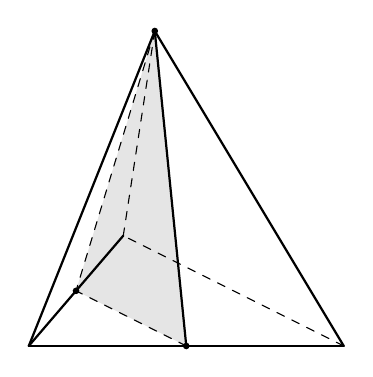
\begin{tikzpicture}[
  scale=1,
  line cap=round,
  line join=round
]
  % Основание
  \coordinate (A) at (0,0);
  \coordinate (B) at (4,0);
  \coordinate (C) at (1.2,1.4);

  % Вершина
  \coordinate (S) at (1.6,4);

  % Средняя линия основания
  \coordinate (M) at (2,0);      % середина AB
  \coordinate (N) at (0.6,0.7);  % середина AC

  % Полупрозрачная секущая плоскость
  \fill[black!10] (S)--(M)--(N)--cycle;

  % Основание пирамиды
  \draw[thick] (A)--(B);
  \draw[thick] (A)--(C);
  \draw[dashed] (B)--(C);

  % Боковые рёбра
  \draw[thick] (S)--(A);
  \draw[thick] (S)--(B);
  \draw[dashed] (S)--(C);

  % Грани отсечённой пирамиды / след плоскости
  \draw[thick] (S)--(M);
  \draw[dashed] (S)--(N);
  \draw[dashed] (M)--(N);

  \fill (S) circle (1.2pt);
  \fill (M) circle (1.2pt);
  \fill (N) circle (1.2pt);
\end{tikzpicture}
}
